\section{Fast Execution on Individual Machines}
\label{sec:multicore}


\subsection{Space-filling Curves}

Outline:
\begin{itemize}
\item Define hilbert priority function and general work flow of ordering algorithm
\item Show distribution of vertex ID distance between every pair of neighbors w/ and w/o Hilbert ordering
\item Give rationale for why it exhibits good cache behavior (perhaps show Theorem w/o proof)
\end{itemize}




In this section, we will describe the rationale behind using the
Hilbert space-filling curve as a way of mapping an $N$-dimensional
space onto the real line, specifically to use this mapping as a
priority function for the priority-dag scheduler in \proc{Prism}.
We will present event counters (e.g. cache misses, TLB misses etc.), 
measured performance and span for three serial experiments on the same
set of graphs: chromatic scheduling, priority-dag scheduling with
a random priority function and priority-dag scheduling with a
Hilbert curve priority function.  

\begin{figure}[h]
\centering
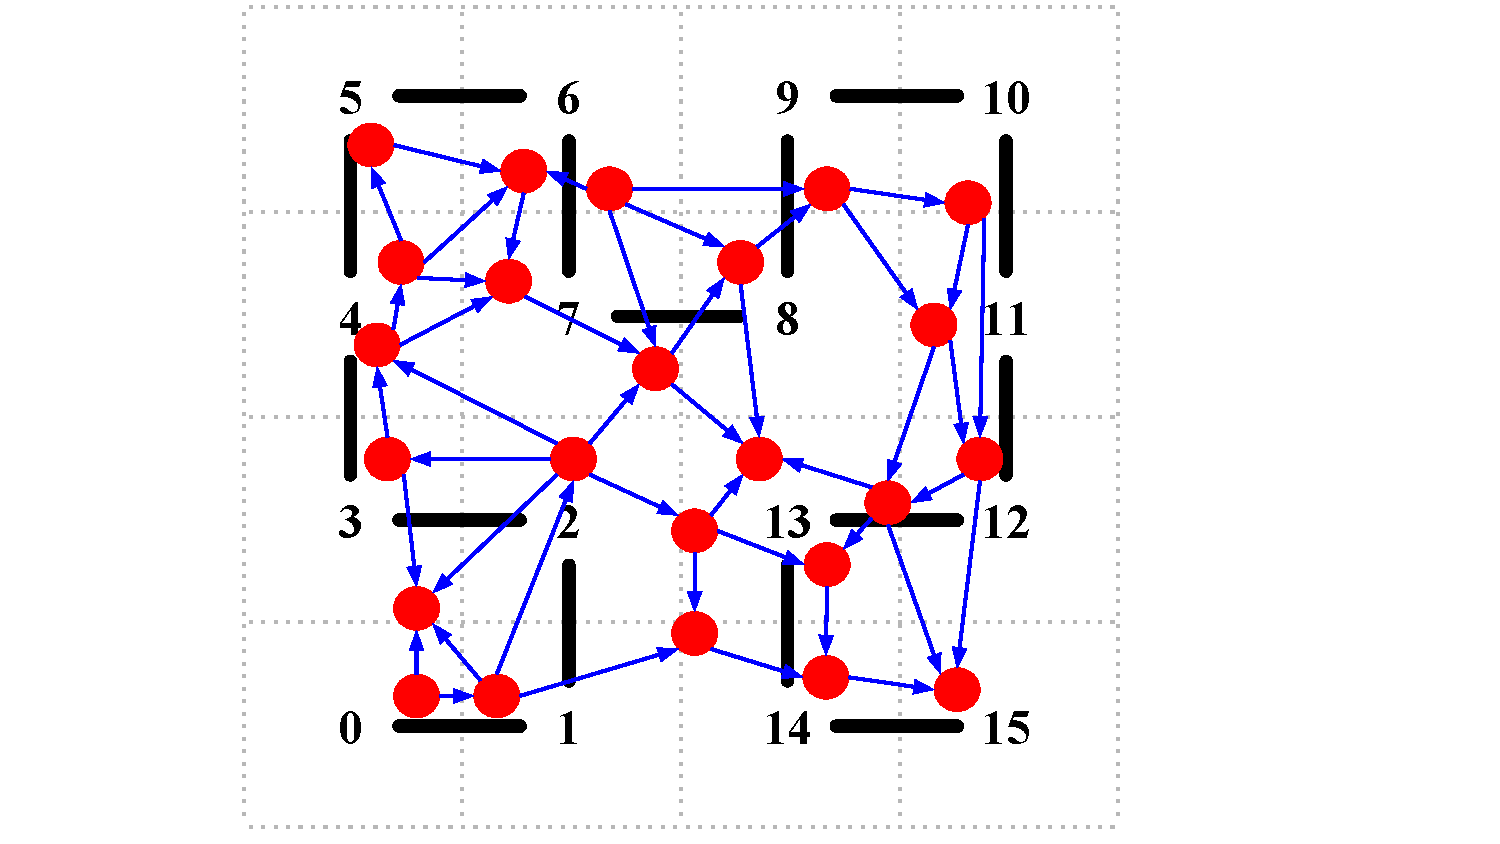
\includegraphics[width=5in]{figures/hilbert_priority_function.pdf}
\caption{Example of how a locally-connected graph in 2 dimensions
is mapped to a dag via the Hilbert priority function.  Each
vertex is mapped to its closest grid point in the discretized
Hilbert curve.  Among vertices mapping to the same Hilbert grid
point, ties are broken randomly.}
\label{fig:hilbert_priority}
\end{figure}


\begin{figure}[h]
\centering
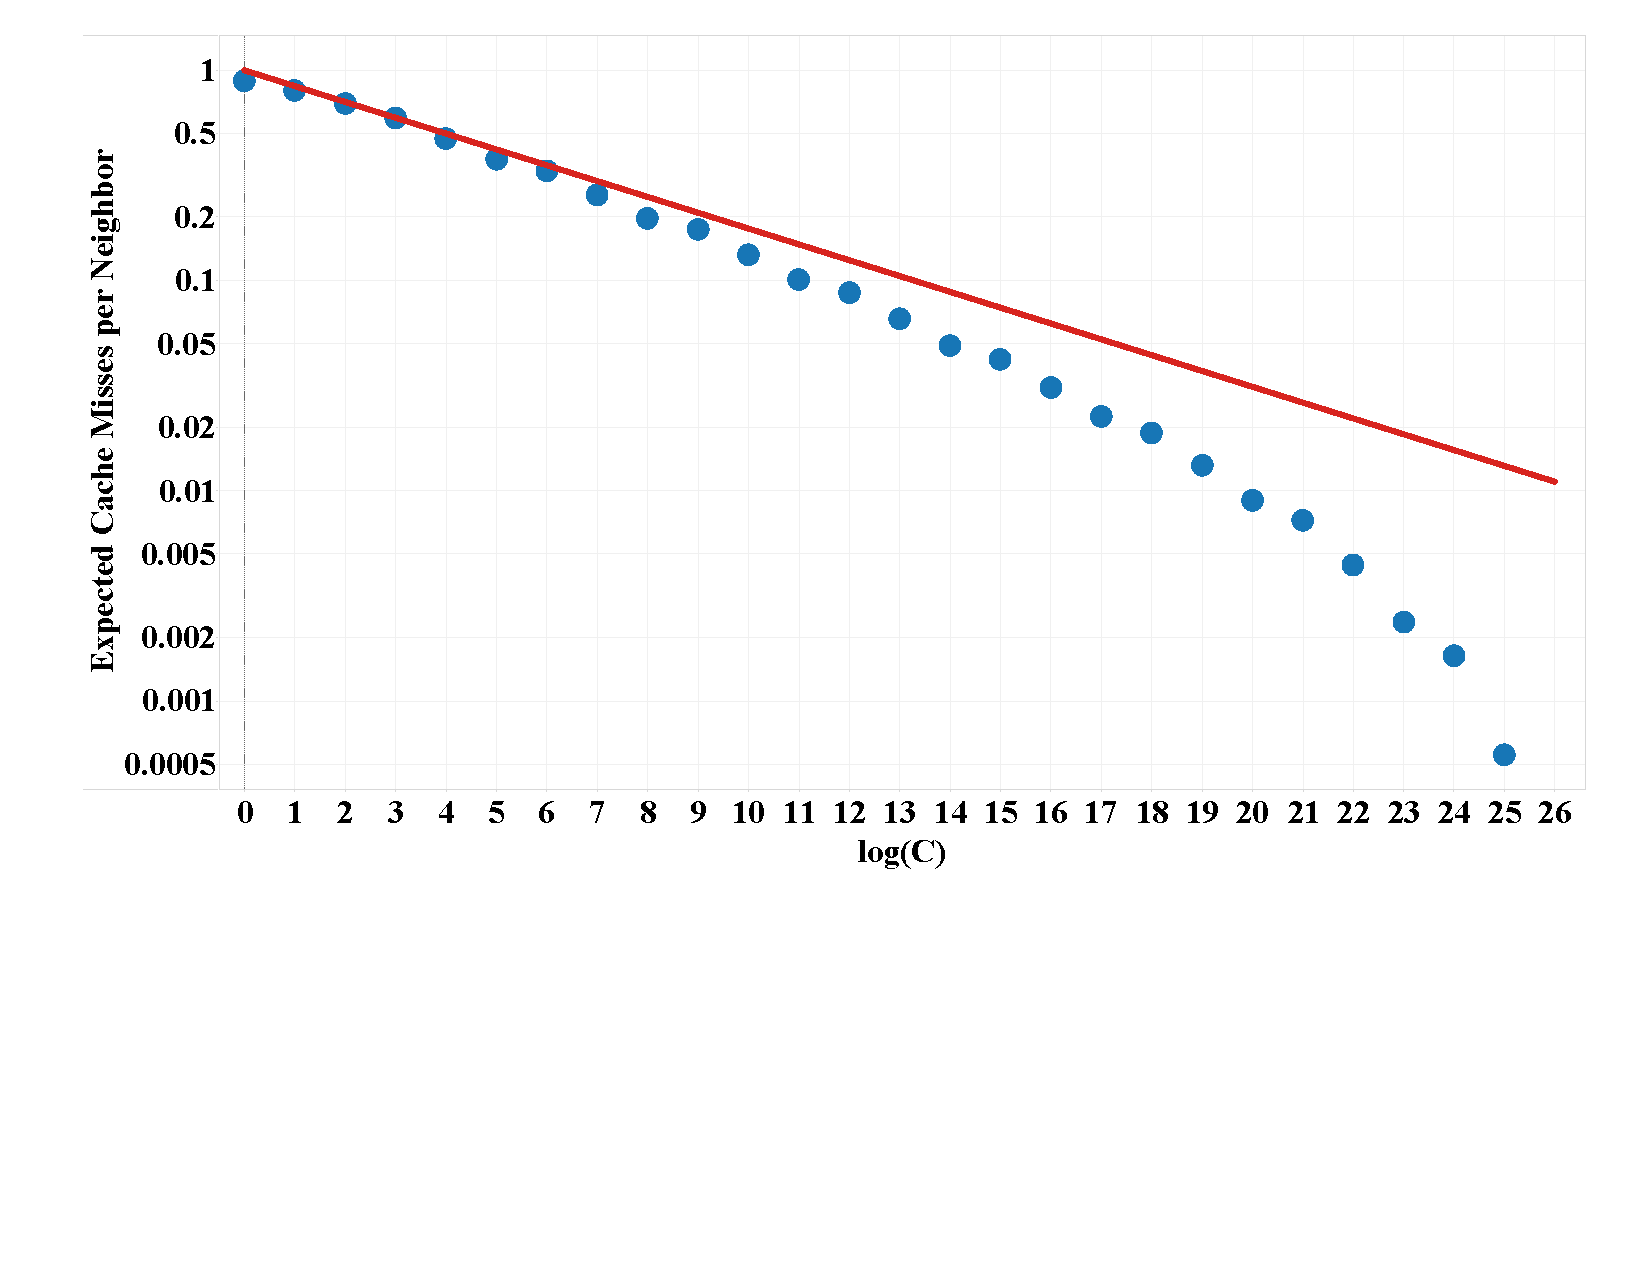
\includegraphics[width=5in,clip,trim=1cm 6cm 0 0]{figures/miss_rate_curve.pdf}
\caption{Miss rate curve...}
\label{fig:miss_rate_curve}
\end{figure}

\begin{figure}[h]
\centering
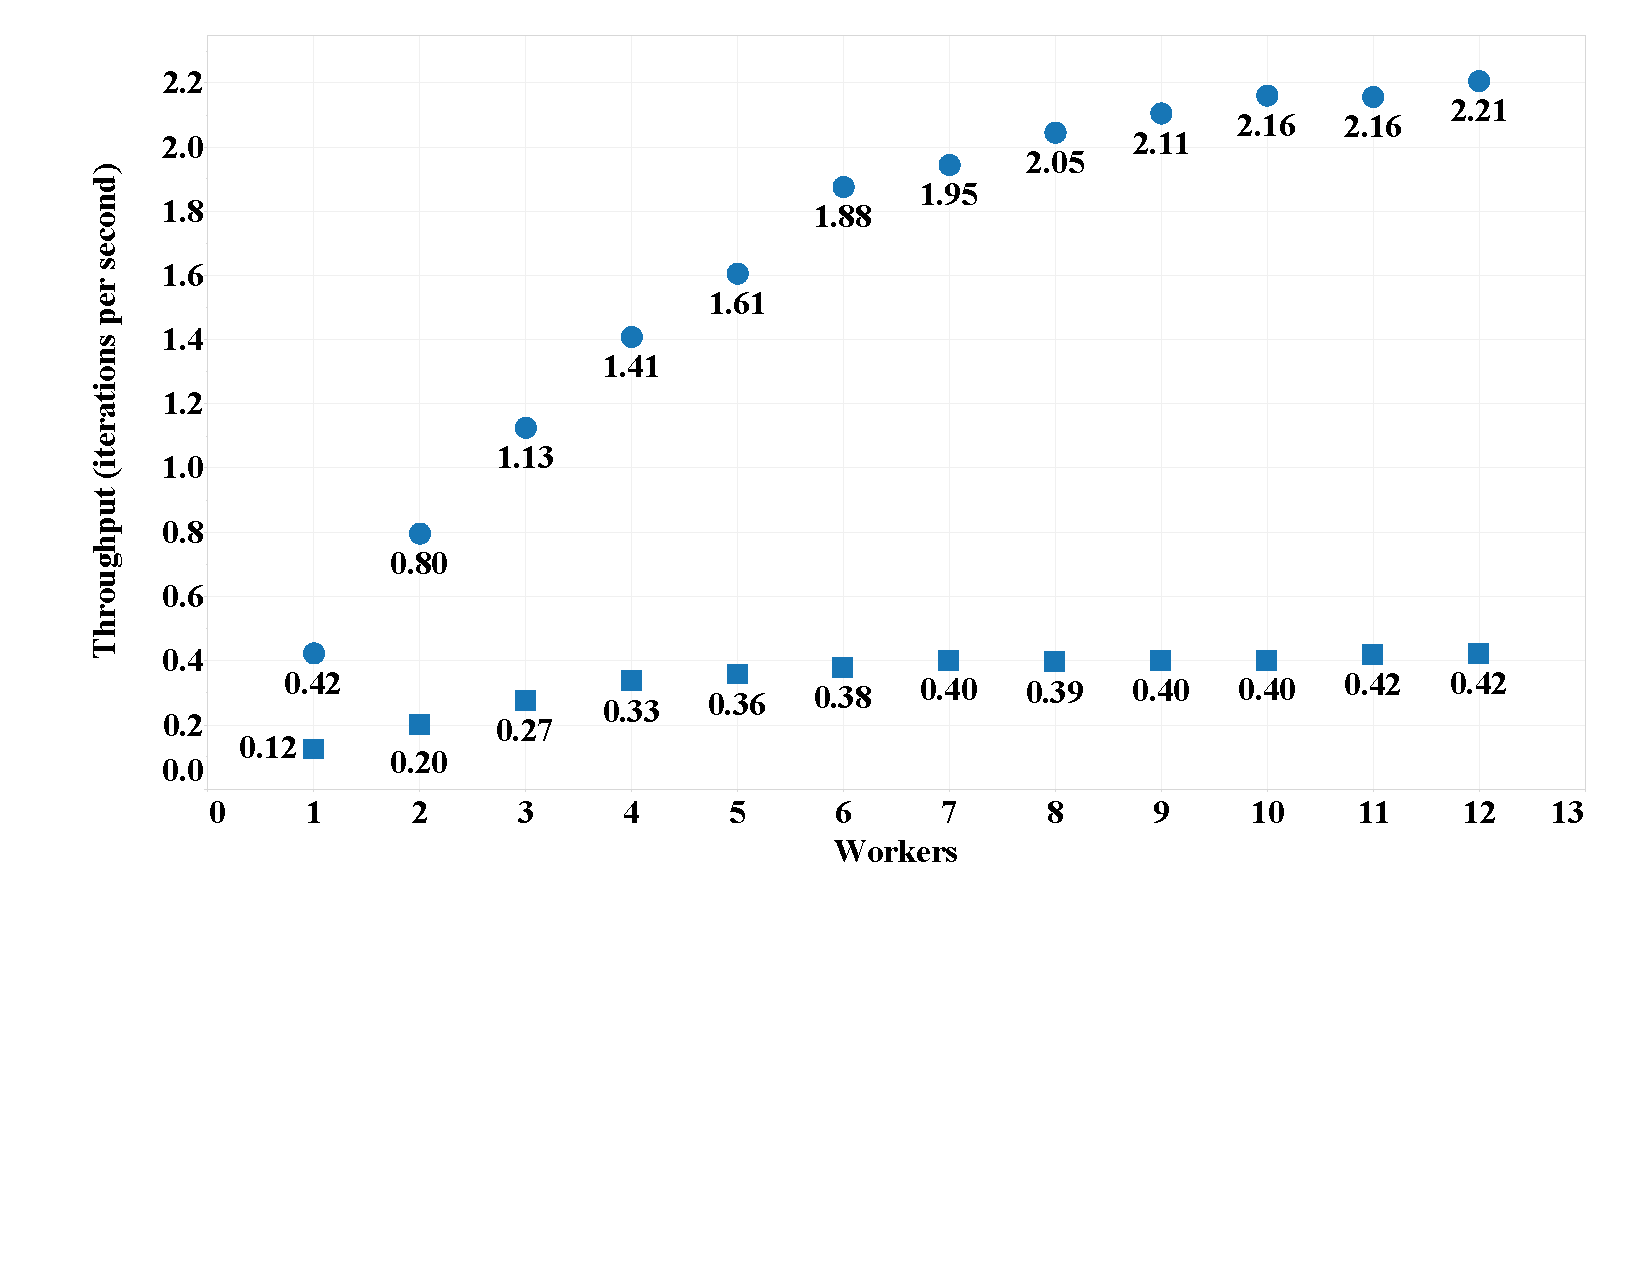
\includegraphics[width=5in,clip,trim=1cm 6cm 0 0]{figures/scalability_bsp.pdf}
\caption{Scalability.}
\label{fig:scalability_bsp}
\end{figure}

\begin{figure}[h]
\centering
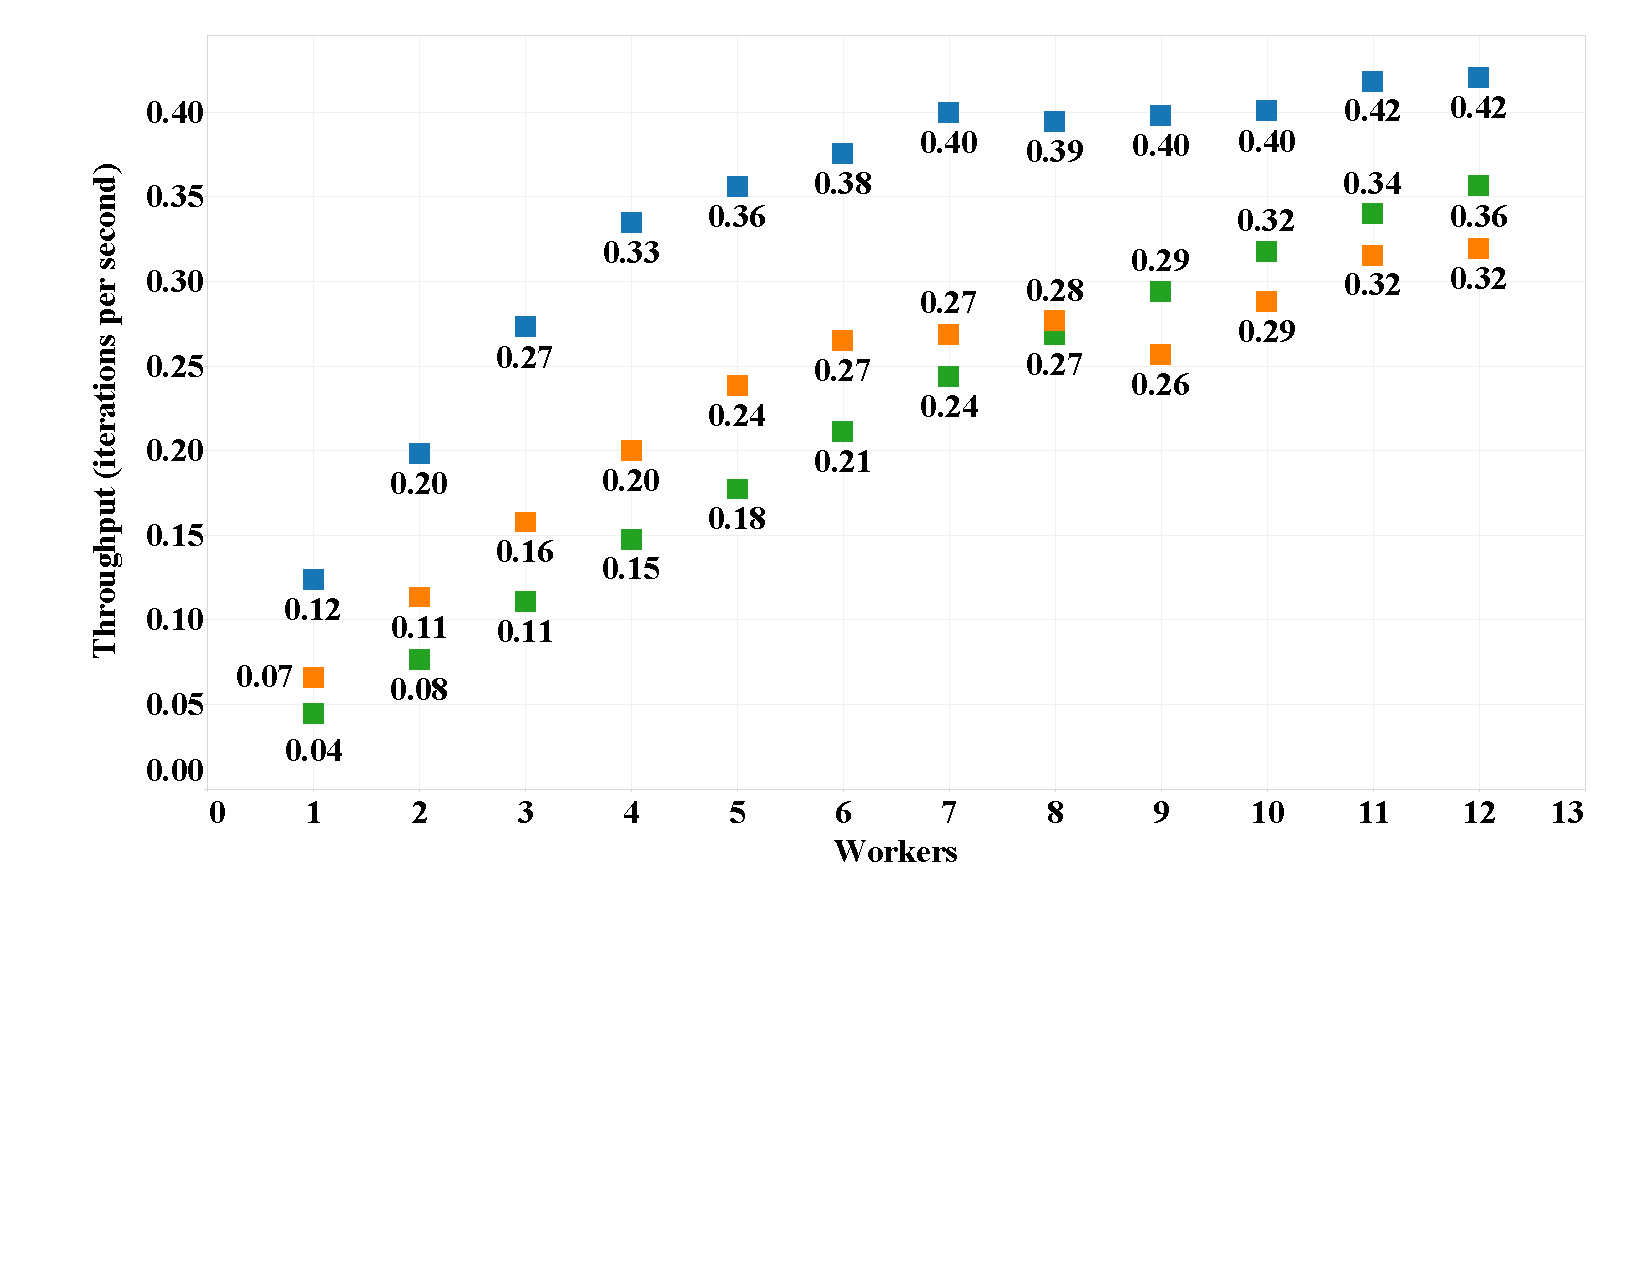
\includegraphics[width=5in,clip,trim=1cm 6cm 0 0]{figures/scalability_original.pdf}
\caption{Scalability.}
\label{fig:scalability_original}
\end{figure}

\begin{figure}[h]
\centering
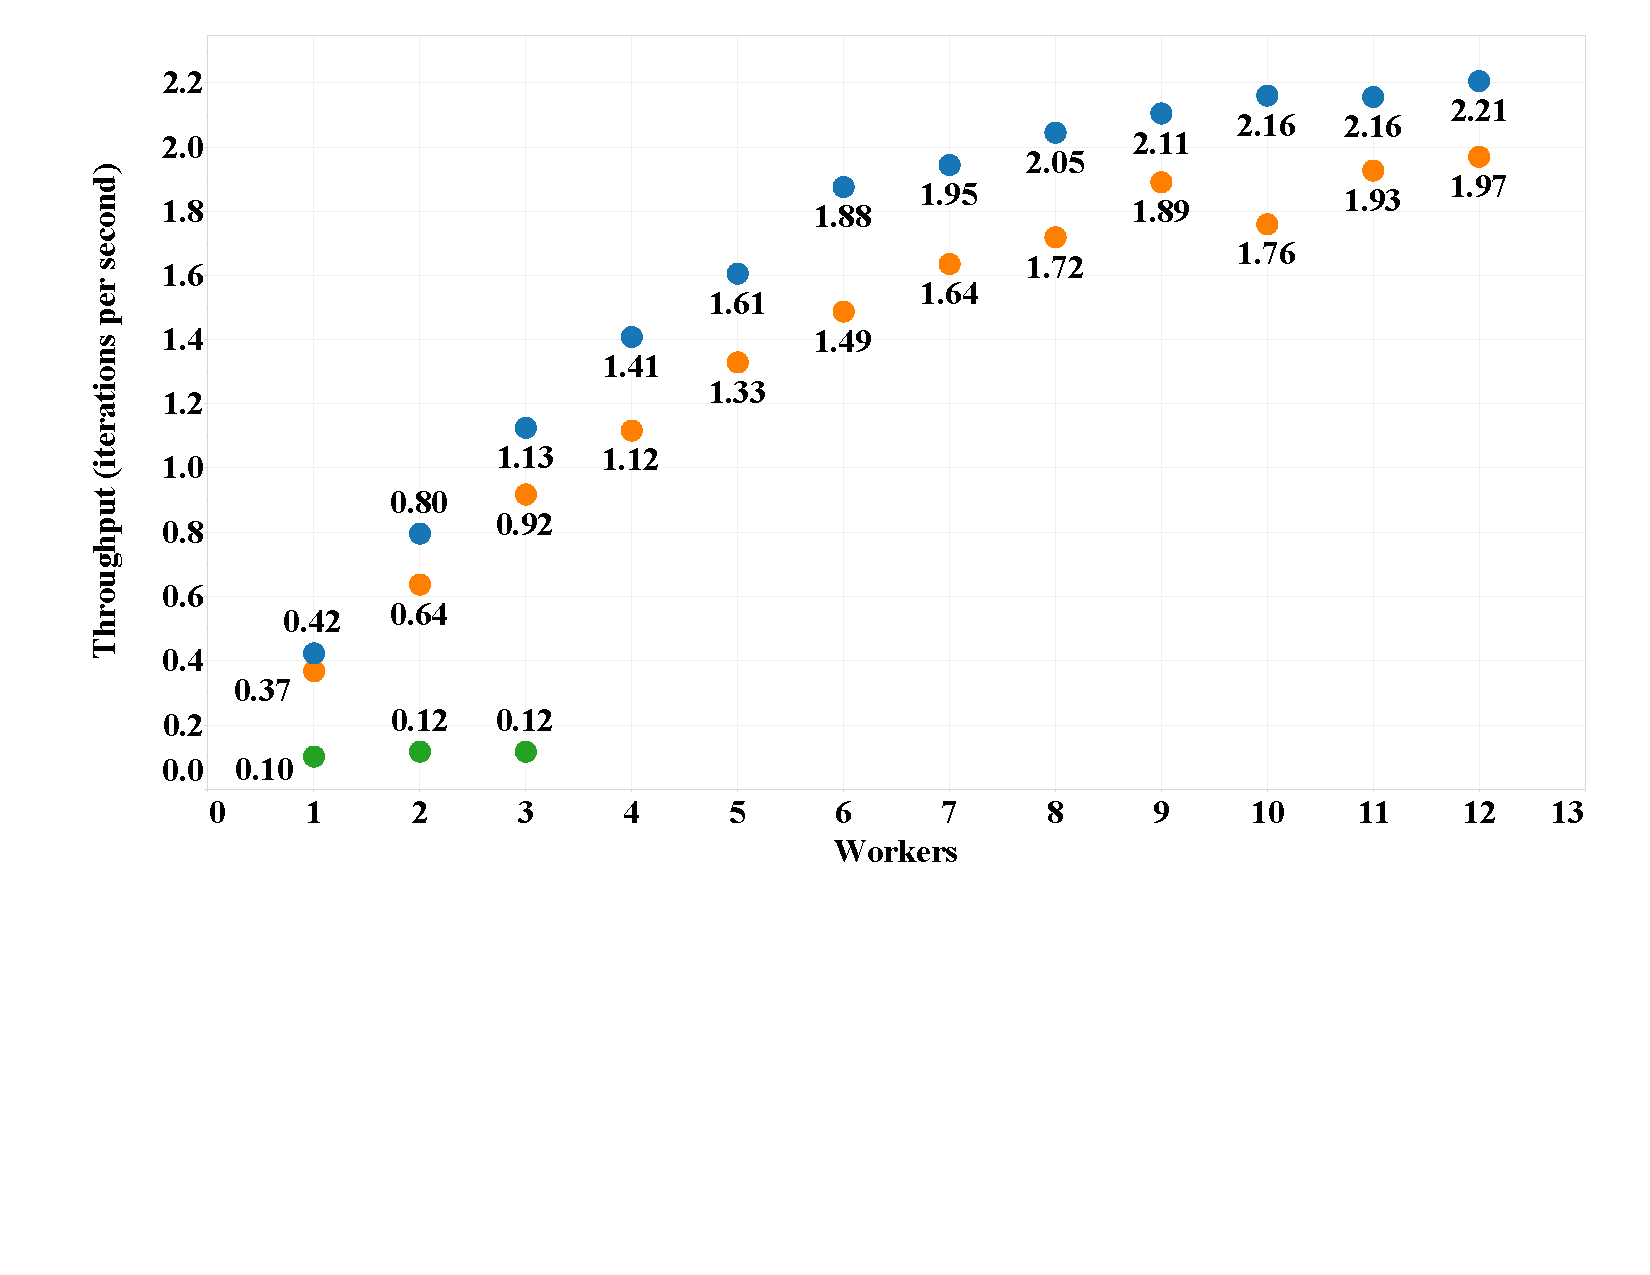
\includegraphics[width=5in,clip,trim=1cm 6cm 0 0]{figures/scalability_reordered.pdf}
\caption{Scalability.}
\label{fig:scalability_reordered}
\end{figure}

\begin{figure}[h]
\centering
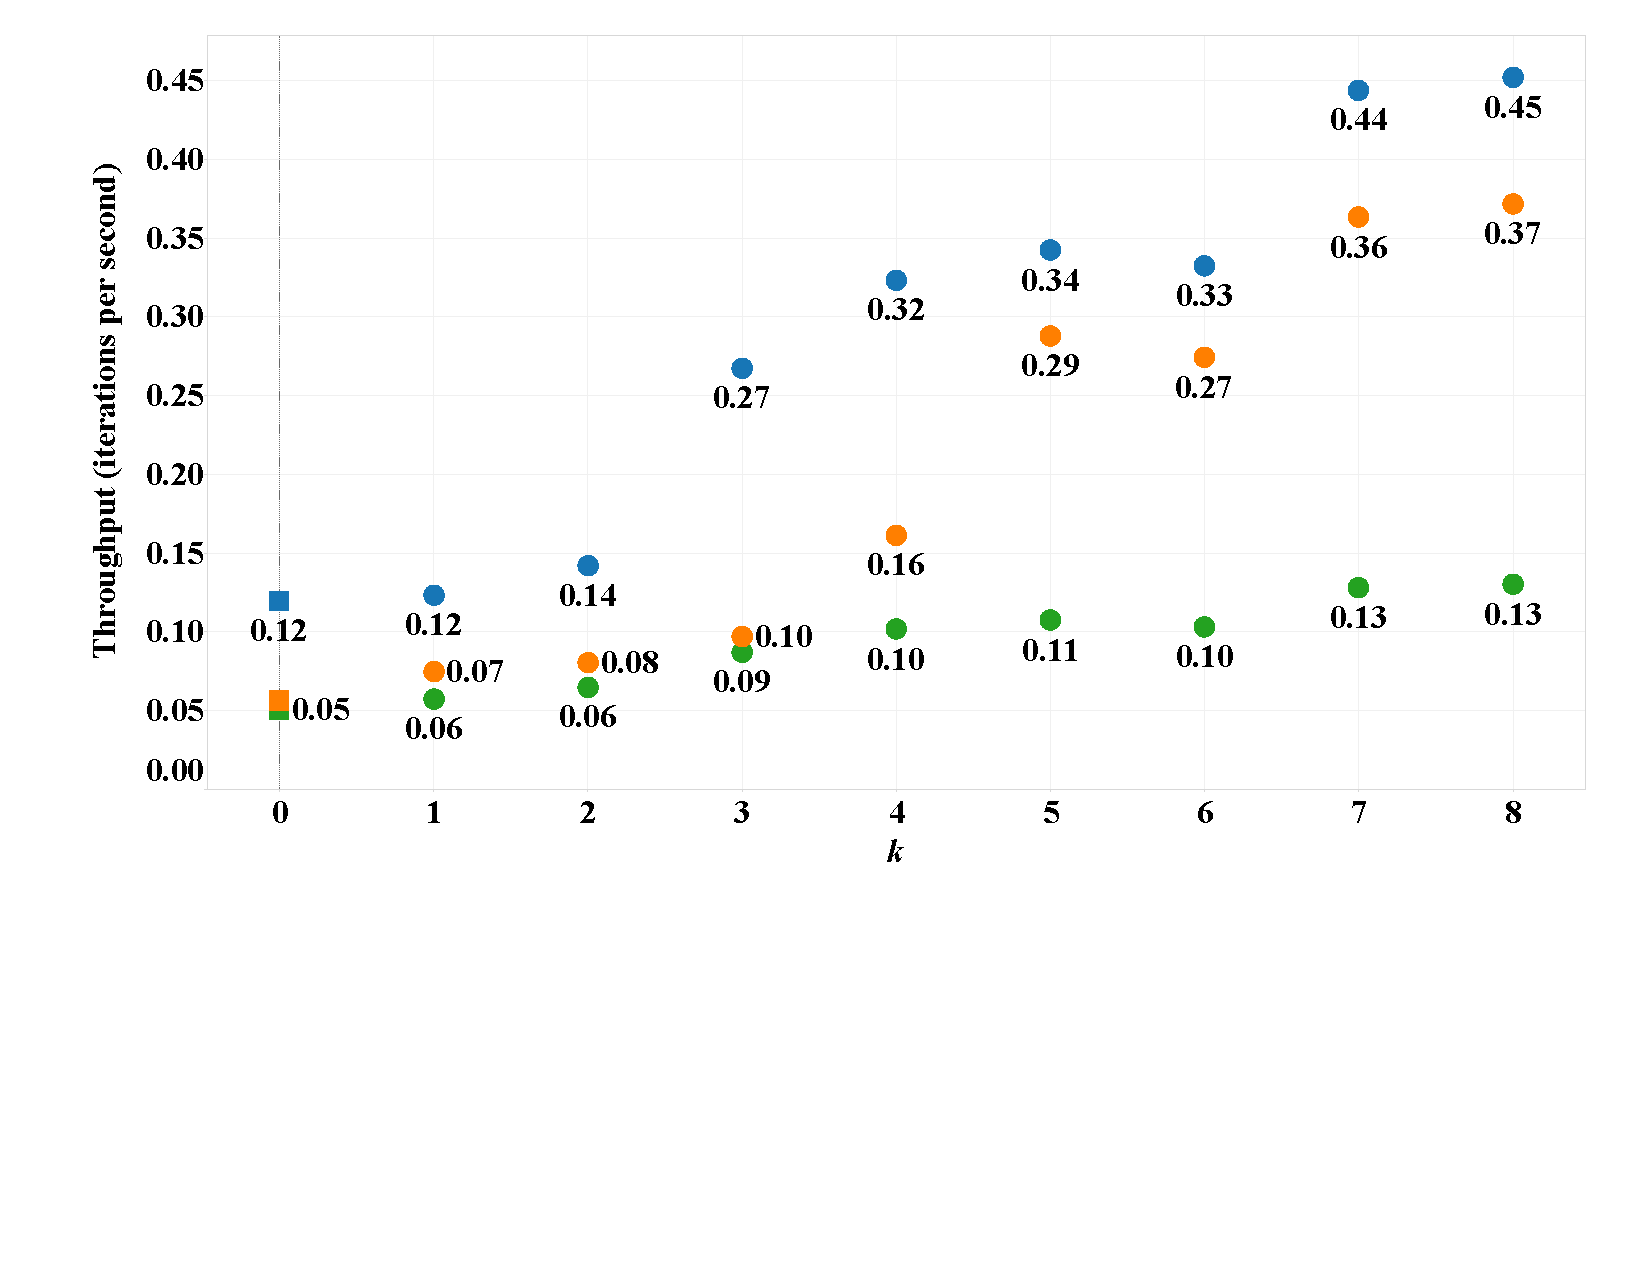
\includegraphics[width=5in,clip,trim=1cm 6cm 0 0]{figures/scalability_hilbert_bits_serial.pdf}
\caption{Scalability.}
\label{fig:scalability_hilbert_bits_serial}
\end{figure}

\begin{figure}[h]
\centering
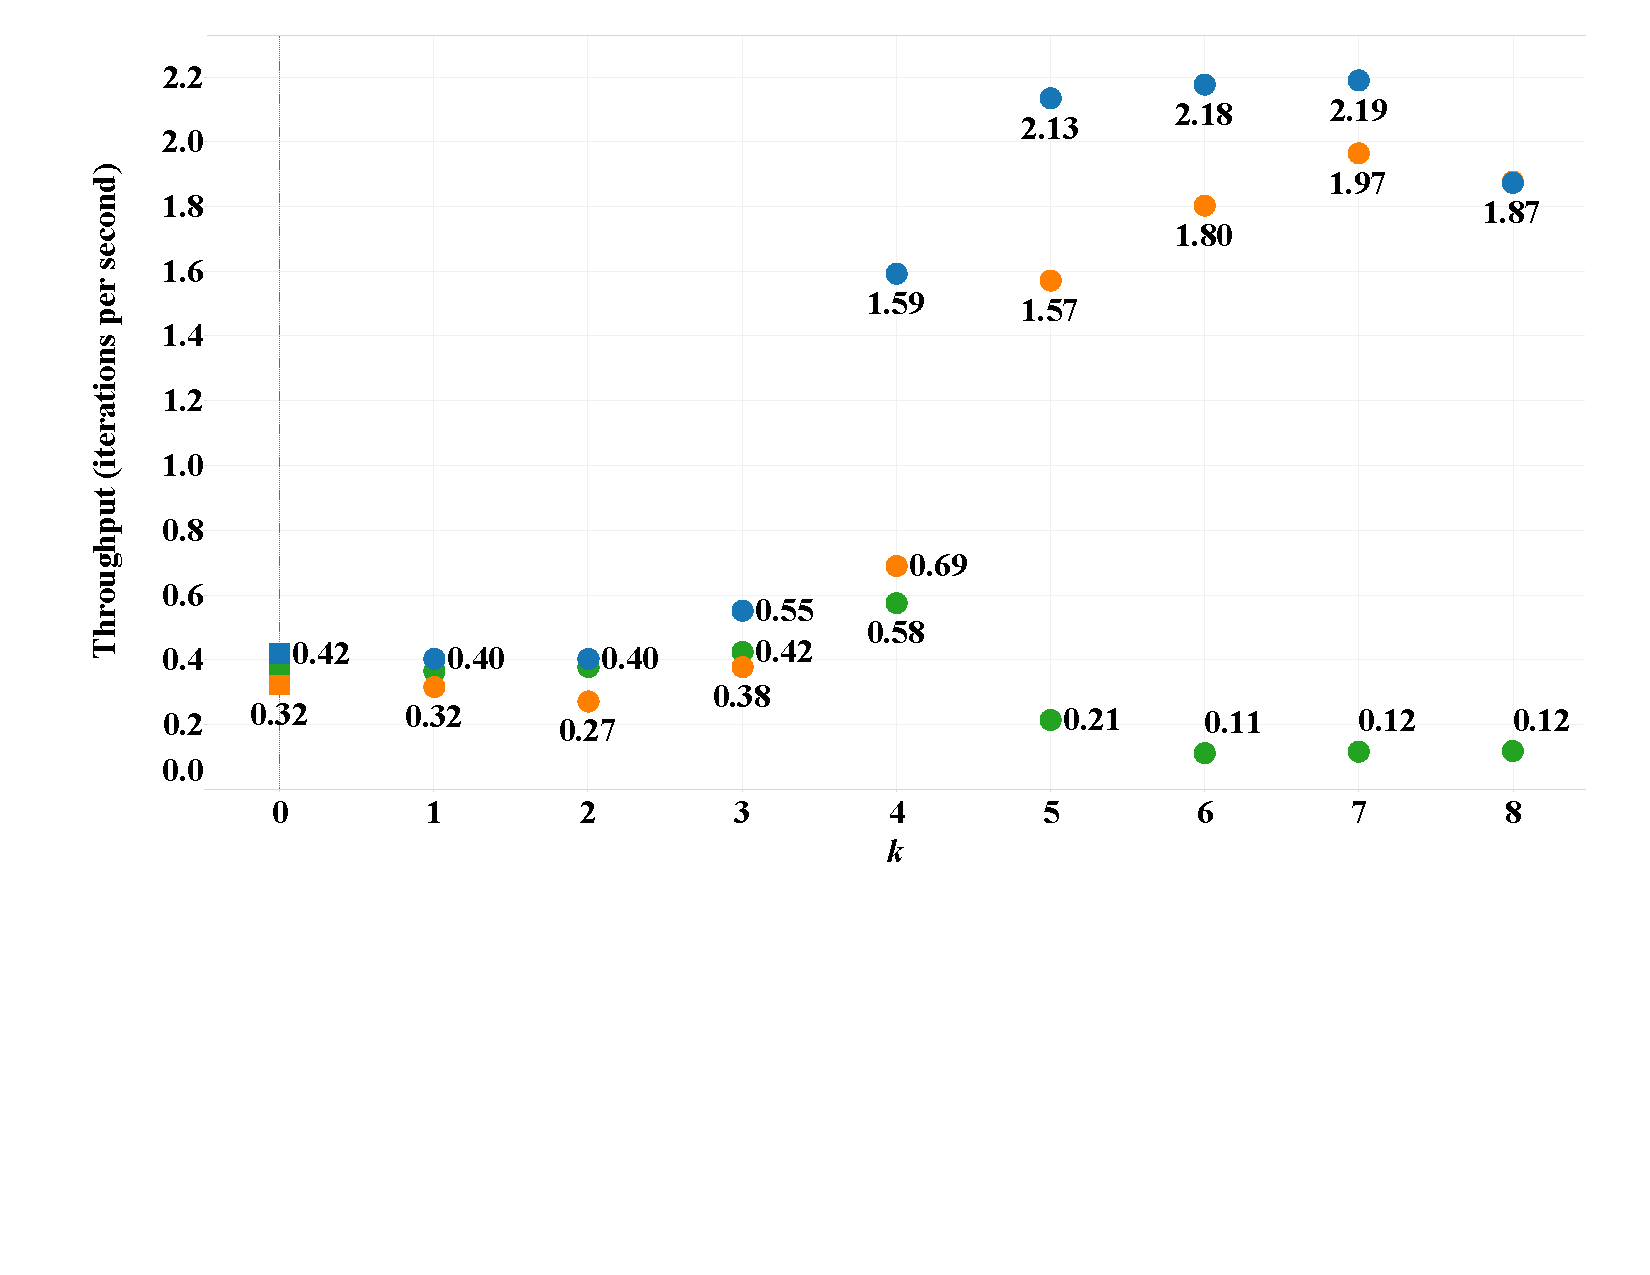
\includegraphics[width=5in,clip,trim=1cm 6cm 0 0]{figures/scalability_hilbert_bits_parallel.pdf}
\caption{Scalability.}
\label{fig:scalability_hilbert_bits_parallel}
\end{figure}



Once we have a good vertex partitioning and a strategy for distributed execution, throughput depends largely on single-machine performance. We explore a number of schemes to this end.


\subsection{Graph Representation in Memory}
We represent graphs in memory on a single machine as follows. We have an array of vertices and an array of edges. Each vertex contains data and a pointer into the edge array indicating the start of its list of edges. Adjacent vertices have adjacent edge lists. Each edge is simply a pointer into the vertex array. This organization is shown in Figure 3.

\subsection{Scheduling for Parallel Execution}
There are two major strategies for scheduling vertices for parallel execution that preserve the appearance of a global ordering across updates and avoid data races. The first is coloring \cite{KalerHaSc14}. If we color a graph so that no two neighboring vertices have the same color, we can safely execute the updates for vertices of the same color in fully in parallel. The reason is that if any vertex's data is being written by some thread, it cannot be read in parallel by another thread because this would require a neighbor of this vertex to be updating concurrently, which is impossible. With the coloring strategy, we sort the vertex array (and the corresponding edge lists) by color and step sequentially through the colors, updating the vertices of each color in a parallel loop.

The other strategy is priority DAG scheduling \cite{JonesPl93}. This involves assigning each vertex a distinct priority, so that we can form a DAG from our graph by adding a direction to each edge such that the source is the endpoint vertex with higher priority. We assign each vertex a counter equal to the number of predcessors it has. We can start by executing all vertices with no predecessors in parallel. Once a vertex is complete, we atomically decrement the counter of each of its successors. If a vertex's counter becomes zero, we can spawn the update of this vertex as another parallel strand of execution. We thus attain fairly high parallelism at the cost of using atomics, which can involve expensive memory barriers on modern hardware. Once again, there can be no data races because two neighboring vertices cannot execute concurrently since one must be the predecessor of the other.

\subsection{Achieving Cache Locality}
If we update the vertices in the vertex array sequentially, as we do with coloring-based scheduling, we get good cache locality (cached lines are processed completely after being fetched) on our accesses to the vertices being updated and to their corresponding entries in the edge array, which is also processed sequentially. Cache locality here includes data cache and TLB locality, since pages in the vertex and edge arrays corresponding to vertices being updated are processed completely after their first access. TLB misses have been shown to be a significant factor in the runtimes of data-intensive computations and are an important consideration for us.

While we get good locality on edge and vertex array accesses for vertices being updated, we get poor locality for accesses to the vertex array to fetch these vertices' neighbors. These accesses are essentially random unless we have sorted the vertex array in some locality-improving manner. Ideally we could store vertices' neighbors close to them in the vertex array. This would confer two benefits. First, TLB misses would fall since neighbors of a vertex will in most cases be stored in the same page as the vertex. Secondly, if a vertex being updated pulled neighbors that were yet to be updated into cache, those neighbors would be updated before they left cache, reducing cache misses.

These considerations suggest that ordering vertices in the vertex array by breadth-first search (BFS) level would be helpful. A vertex at BFS level $n$ can only have neighbors at BFS levels $n-1$ and $n+1$; if there was a neighbor at a smaller level, the vertex would have smaller level than $n$, and there can be no neighbors at levels greater than $n+1$ if the vertex is at $n$. Thus, if BFS levels are fairly small, ordering the vertices by BFS level would result in nearby neighbor accesses as desired. BFS levels are generally bounded in size in mesh graphs; they grow at first, but once the largest cross-section of the mesh is reached, successive levels should have similar size. The problem with ordering the entire vertex array by BFS level is that there are no longer defined sequential regions over which parallel update loops can be run -- since any two adjacent vertices could be neighbors -- so parallelism is lost. We implement and evaluate a hybrid coloring-BFS approach that restores some parallelism while preserving our locality wins: within each BFS level, we sort by color, so that within each BFS level we can update the vertices of each color in parallel. The BFS levels are executed sequentially. This scheme brings up an important point about the locality-parallelism design space -- after a point, increasing parallelism is not necessarily important. If there is enough parallelism to saturate the cores of the available machines, locality is likely the parameter worth optimizing.

% Analyze for priority DAG case
In the case of priority DAG scheduling, cache behavior is very different. We lose the locality of access to the vertex and edge arrays for vertices being updated that we have in the sequential processing case. But we are not without victories: when we update the last predecessor of some node we immediately afterwards update that node, at which point is hot in cache. So accesses to neighbors of vertices being updated do not have worst-case cache behavior as they do in the sequential processing case.

For ideal cache behavior, the story is similar to the sequential processing case. We would like for neighborhoods of nearby vertices to be stored fairly contiguously in the vertex array so that accesses to neighbors of vertices being updated tend not to cause TLB misses. We would also like these neighborhoods to be updated completely in some small time window so that fetched neighbors are updated before they leave cache. Achieving the first objective is possible by using a BFS-based ordering or by preserving the Z-number ordering described above for partitioning vertices across machines. We take the second approach because BFS levels may be larger than memory pages and therefore TLB misses are more likely under the BFS-based ordering. Achieving the second objective is much harder with DAG scheduling because the order in which vertices are updated is unclear. However, if we assign each vertex a priority equal to its Z-number, we suspect that if we spawn off the processing of vertices with no predecssors in order of Z-number and if we can assume that earlier spawned routines tend to execute to completion before later spawned routines begin executing (as is the case in the Cilk model of multithreading), then contiguous regions of the physical mesh should be processed nearly to completion in small periods of time. 

% "small period of time" is not precise...

%Draw parallel to cache-oblivious?

\subsection{Considering Parallelism}
% atomics, barriers in the priority DAG case
% cache transfers across processors are fast -- so as long as the data is in some cache, we are OK (not for TLB though) ... BUT
% Cilk -- steals high in the tree

\subsection{Prefetching}
